% !Mode:: "TeX:UTF-8"
%% 请使用 XeLaTeX 编译本文.
% \documentclass{WHUBachelor}% 选项 forprint: 交付打印时添加, 避免彩色链接字迹打印偏淡. 即使用下一行:
 \documentclass[forprint]{WHUBachelor}
\usepackage{cite} 
\usepackage{amsmath, amsfonts, amssymb} % math equations, symbols
\usepackage[english]{babel}
\usepackage{color}      % color content
\usepackage{graphicx}   % import figures
\usepackage{url}        % hyperlinks
\usepackage{bm}         % bold type for equations
\usepackage{multirow}
\usepackage{booktabs}
\usepackage{epstopdf}
\usepackage{epsfig}
\usepackage{algorithm}
\usepackage{algorithmic}
\usepackage{esvect}
\usepackage{listings}
\usepackage[framed,numbered,autolinebreaks,useliterate]{mcode}
\usepackage{subfig}
\usepackage{float}
\begin{document}
%%%%%%% 下面的内容, 据实填空.


\StudentNumber{力6} % 填写自己的学号

\title{\\有限元法基础\\桥梁设计竞赛报告}

\advisor{张雄教授}

\author{毕恺峰$\,$ 胡昌平$\,$ 黄轩宇 $\,$易泽吉$\,$张逸葑}                            % 作者名字

\Cmajor{工程力学}                  % 专业中文名

\Cschoolname{航天航空学院}          % 学院名

\date{二〇一八年三月}                    % 日期, 要注意和英文日期一致!!


%-----------------------------------------------------------------------------
\pdfbookmark[0]{封面}{title}         % 封面页加到 pdf 书签
\maketitle
\frontmatter
\pagenumbering{Roman}              % 正文之前的页码用大写罗马字母编号.
%-----------------------------------------------------------------------------

%==========================把目录加入到书签==============================%%%%%%
\pdfbookmark[0]{目录}{toc}

\mainmatter %% 以下是正文、
\tableofcontents

\chapter{桥梁的基本选择与设计思路}
\section{悬索斜拉桥}
\subsection{设计思路及设计参数}
悬索斜拉桥是实际工程中对跨度较大的桥的一种设计方案。考虑到题目要求,桥孔最小宽度为150米,为了尽量减小桥面位移,因此将跨度设计为160米,即每160米安装一个桥墩并牵拉斜拉索,一共设置9个桥墩以及斜拉索结构。实际测试中发现,如果斜拉索足够密,则无需桁架结构即可将桥面竖直位移控制在一个较小的值,从而大大降低成本。因此设计时大体控制5米设计一个斜拉索,每个桥墩牵拉4*13根斜拉索。估算整个桥梁的重量及10kPa的均匀载荷引起的竖直方向力的大小约为300MN量级。则每个桥墩所需载重为30MN量级。混凝土许用应力的80\%为18MPa,即每个桥墩的截面积应当大于2平方米的量级。实际设计时,每个桥墩的截面积为12.8平方米。同理,拉索的截面积估算应当大于0.001平方米的量级。实际取为0.0025平方米。
\begin{figure}[H]
\centering  
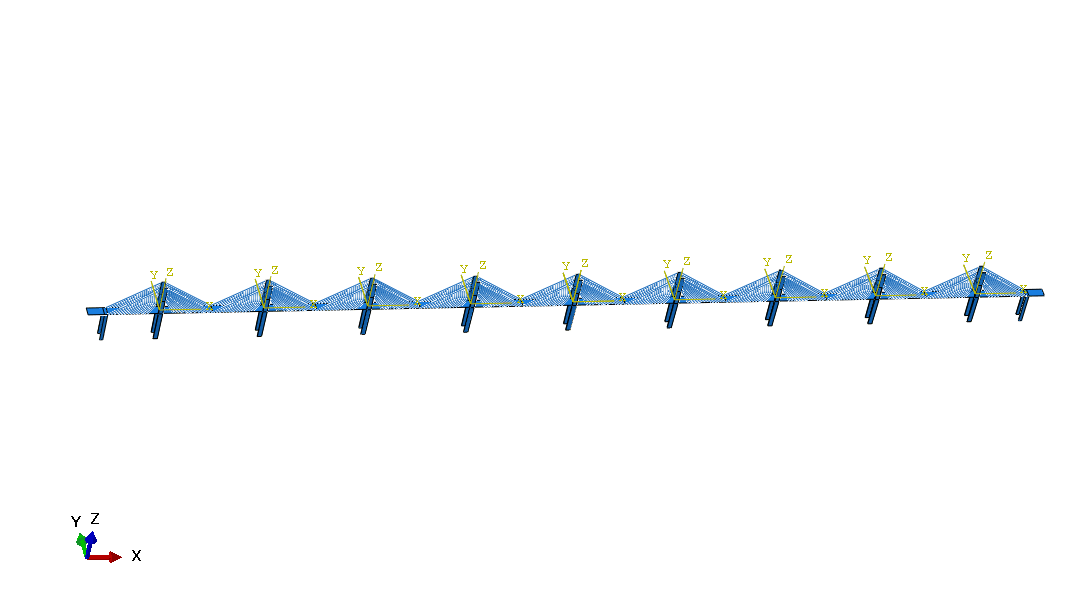
\includegraphics[width = .8\textwidth]{assembly.png} 
\caption{装配图} 
\label{3-1} 
\end{figure}

\subsection{运算结果}
运算结果得到桥面最大位移为0.2843米,斜拉索最大米塞斯应力为266.7MPa,因而斜拉索的米塞斯应力小于钢的许用应力的80\%,即钢的部分无危险区。针对混凝土部分,将色卡上限设为1.8e7(即18MPa),得到的应力云图中未发现有混凝土有超出此应力的部分,即混凝土部分也无危险区。得到的结果如图所示。

\begin{figure}[H]
\centering  
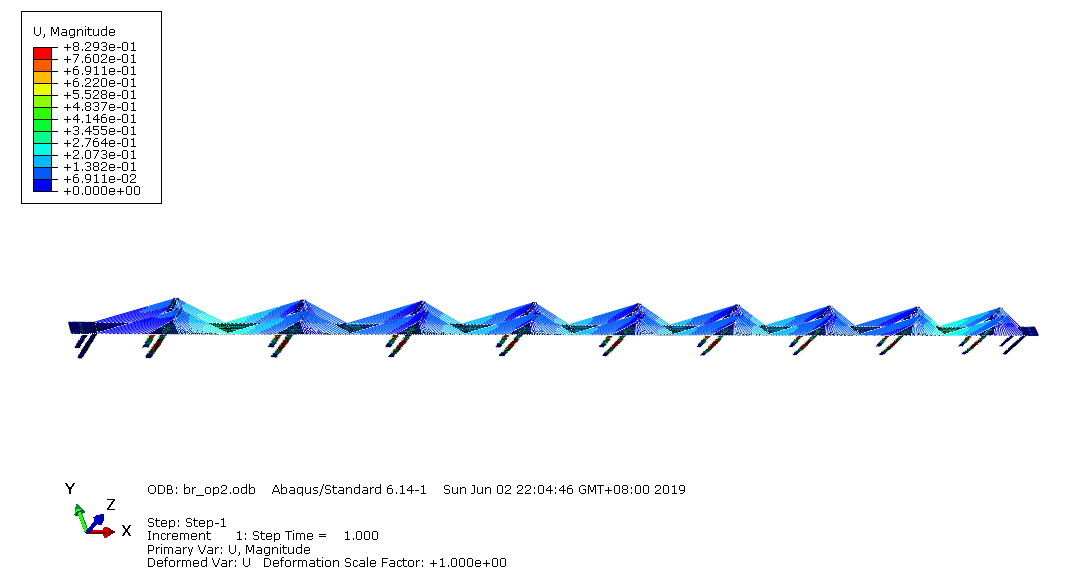
\includegraphics[width = .8\textwidth]{Magnitude.png} 
\caption{位移图} 
\label{3-1} 
\end{figure}

\begin{figure}[H]
\centering  
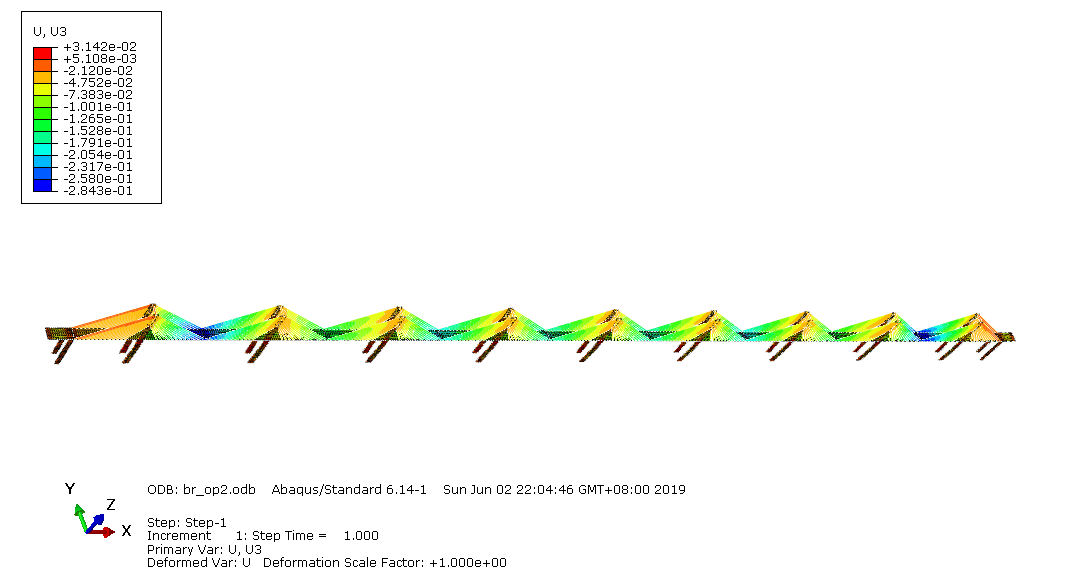
\includegraphics[width = .8\textwidth]{Magnitude3.png} 
\caption{竖直位移图} 
\label{3-1} 
\end{figure}

\begin{figure}[H]
\centering  
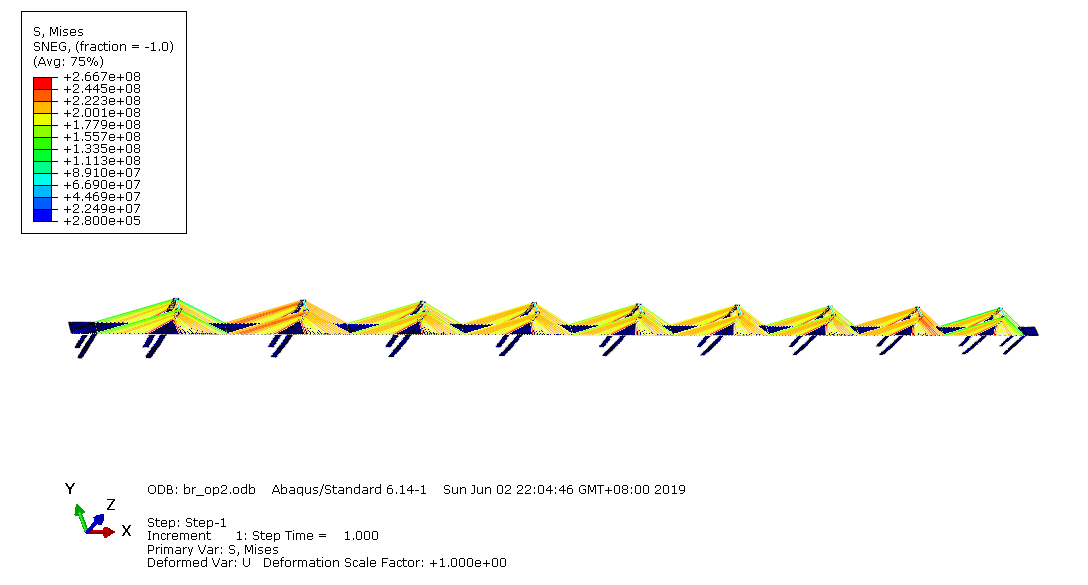
\includegraphics[width = .8\textwidth]{MisesGlobal.png} 
\caption{米塞斯应力云图} 
\label{3-1} 
\end{figure}

\begin{figure}[H]
\centering  
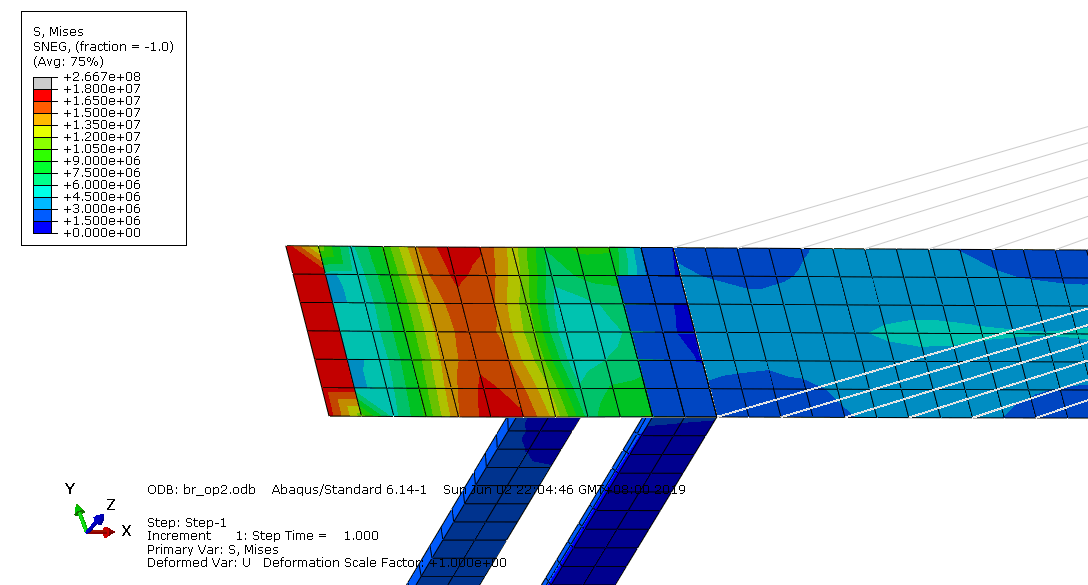
\includegraphics[width = .8\textwidth]{MisesConcrete1.8MPa.png} 
\caption{混凝土米塞斯应力云图(部分)} 
\label{3-1} 
\end{figure}

\section{悬索斜拉桥设计总结}
在实际画桥时,主要的难点在于约束的设定。在Abaqus中,为选定约束集,应当在Part中选定合适的点集,从而在Assembly后继承。在选定约束时,可以选取对应的点集相约束,注意两个点集的点数应当相同,如此可以大大减小工作量。进一步更可将各相同的约束的两个电集设为相似的名字,在脚本中使用循环编写约束。在实际操作中,应当仔细设定网格大小,从而使得对应的约束点可以在浮点数误差内重合,从而和stap++对接。然而我们的桥梁设计主要是为了完成特定考核要求,并未考虑到结构的避震性能、稳定性等因素。因此我们所设计的桥梁与工程实际还是有很大出入的。

\section{拱形箱梁桥}
箱梁是桥梁工程中梁的一种,内部为空心状,上部两侧有翼缘,类似箱子,因而得名。分单箱、多箱等。箱梁在桥梁工程中极为常用,如高架桥、铁路桥中。箱梁可以减少材料的使用,并且提高结构的刚度。钢板箱形梁是工程中常采用的结构形式。为研究横隔板间距对集中荷载作用下简支钢箱梁畸变的影响,通过设置不同数量横隔板的简支钢箱梁,比较其在集中荷载作用下的畸变效应和刚性扭转效应,得到最大畸变效应随横隔板数量的变化曲线在箱梁腹板顶端施加集中荷载,按畸变、刚性扭转、对称弯曲和偏心荷载四种工况采用荷载分解的方法进行计算。箱梁结构如下图所示。

\begin{figure}[H]
\centering  
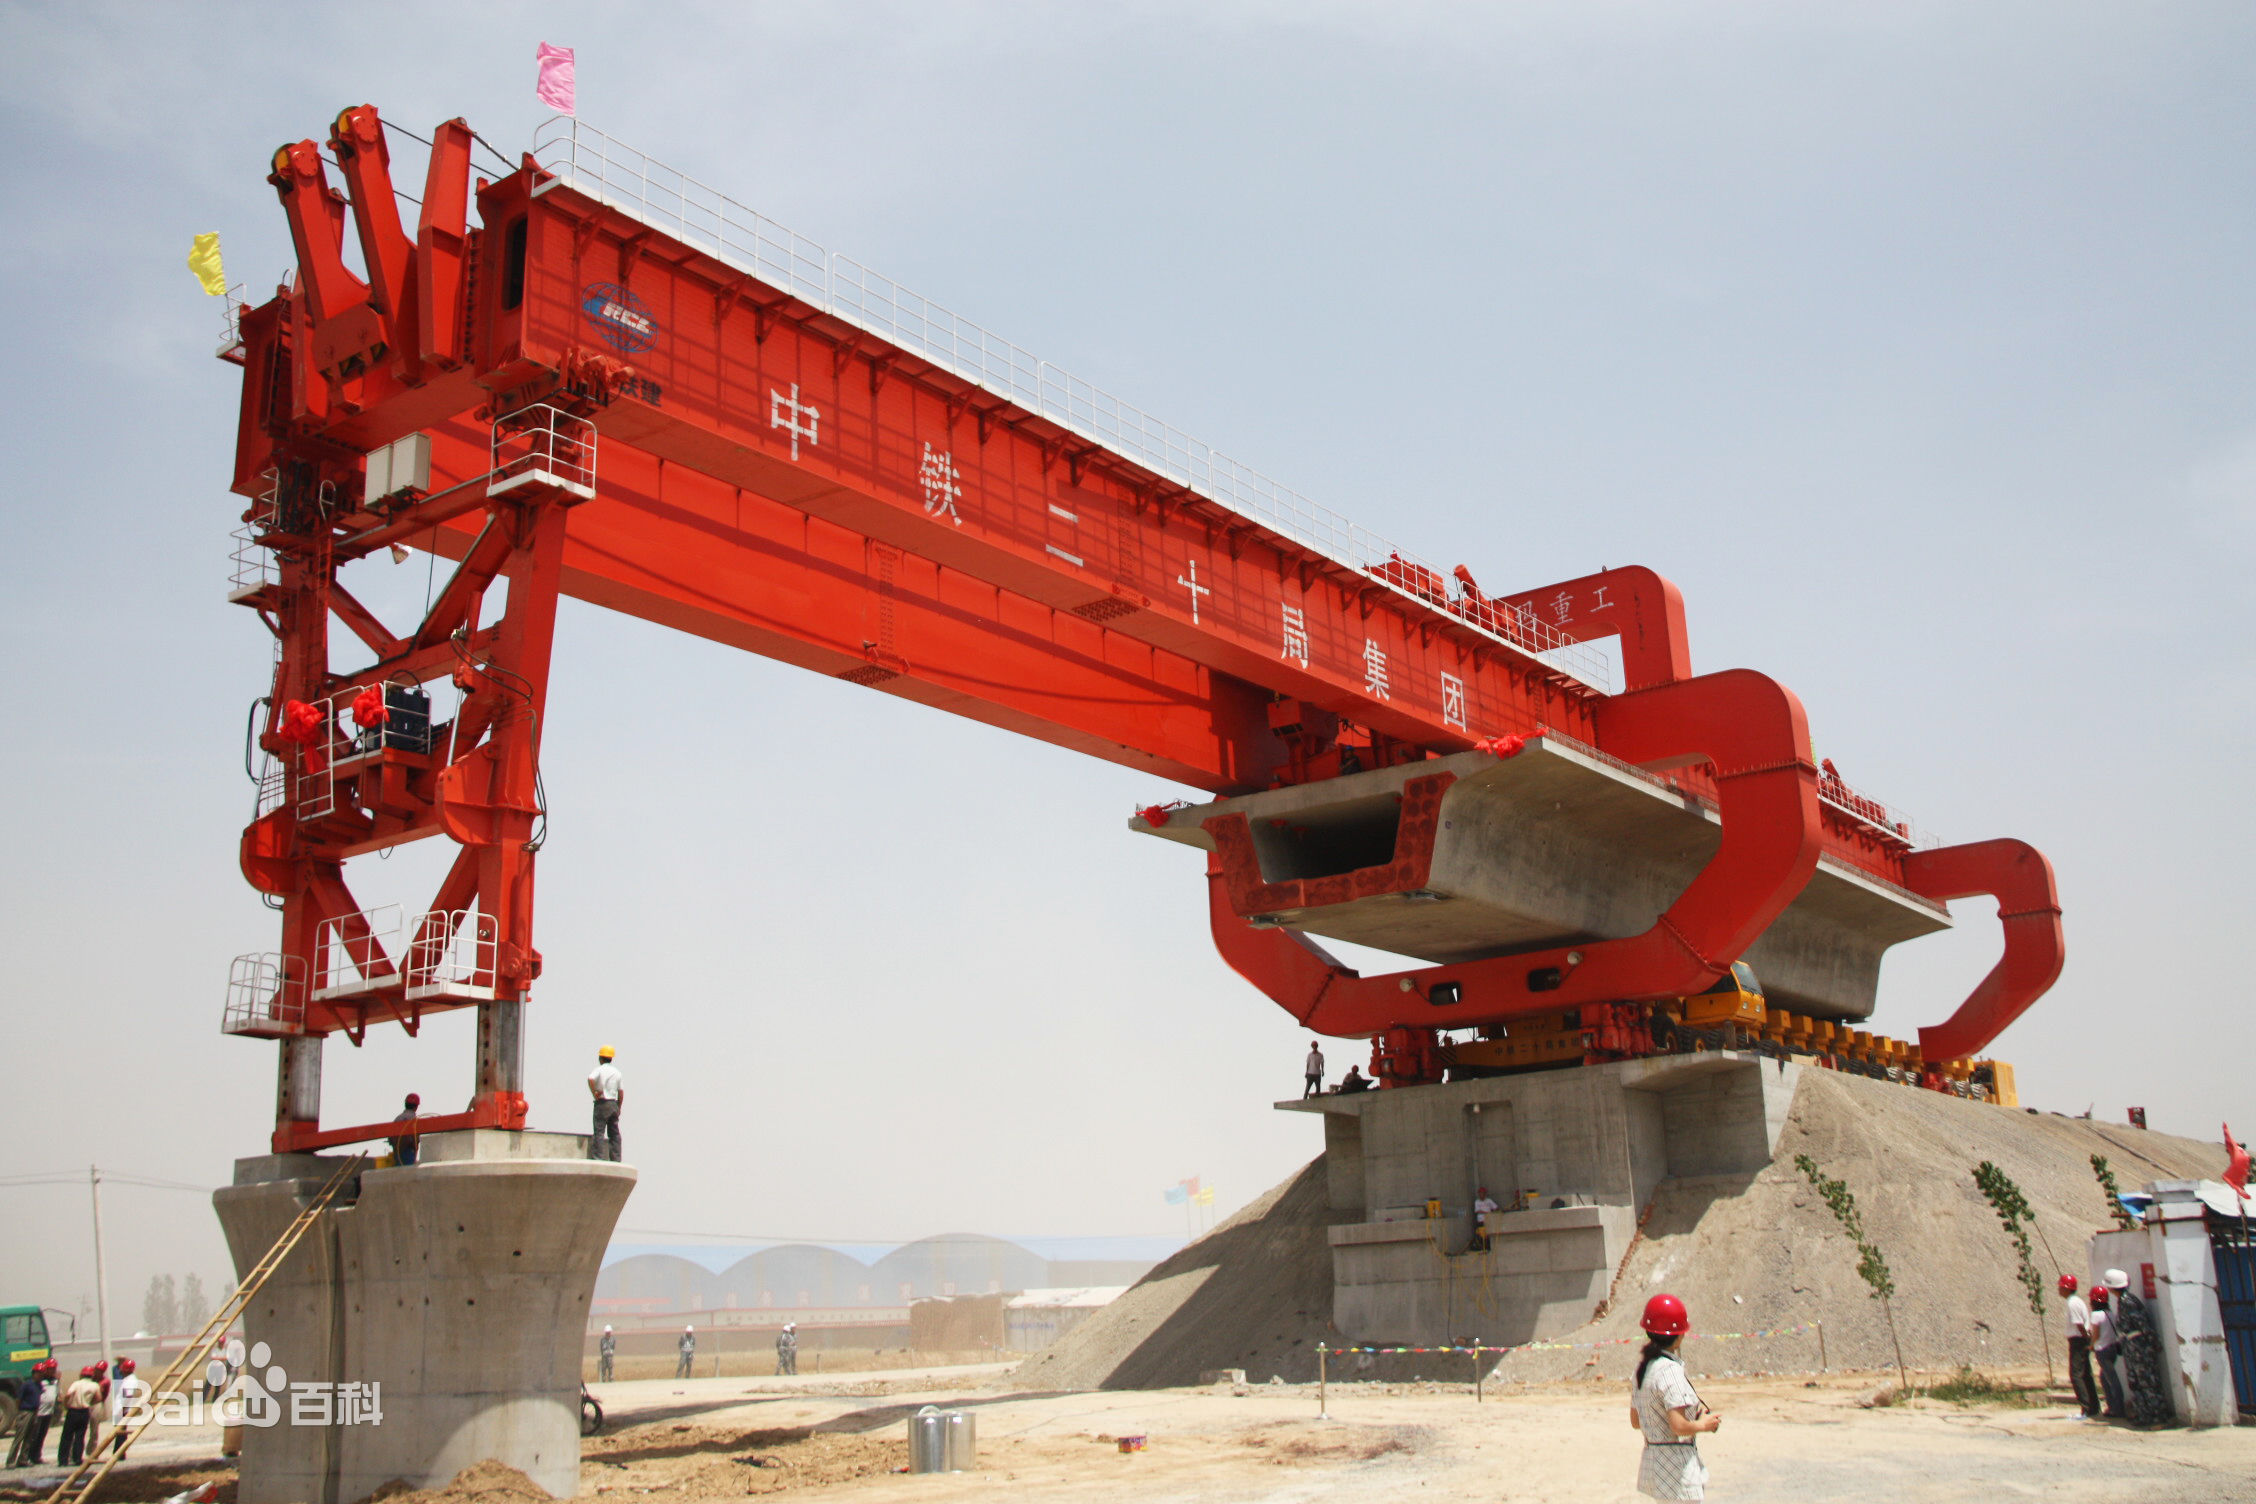
\includegraphics[width = .8\textwidth]{box.jpg} 
\caption{箱梁结构} 
\label{3-1} 
\end{figure}

实际在工程中,架设在桥面底下的箱梁截面积并非不变,而是在距离桥墩近的地方较厚,而距离桥墩较远的地方较薄,类似拱形桥。经验上,支点梁高1/18-1/16,跨中梁高1/50。在设计桥墩时,可以采用双薄壁墩。变梁高的箱梁以及采用双薄壁墩的一个例子如下图所示。

\begin{figure}[H]
\centering  
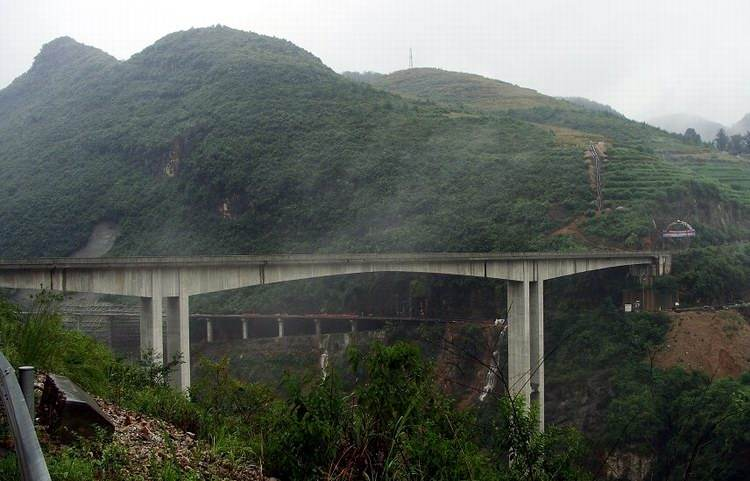
\includegraphics[width = .8\textwidth]{boxexample.jpeg} 
\caption{箱梁结构实例} 
\label{3-1} 
\end{figure}

在实际工程中,应当使用预应力混凝土钢筋结构。但是在Abaqus软件中,使用这种结构较为麻烦,且在我们的stap++程序中并没有相关功能,因此放弃钢筋混凝土结构。直接使用钢筋完成了一个箱梁,梁高恒定为5米,每6米一个梯形梁作支撑,桥跨度为150米。这种简易的箱梁结构在的限元运算结果不甚理想,其桥面最大位移高达9米左右,因此放弃了此设计。

\section{桁架梁桥}

本组设计的梁桥采取多跨上承式桁架梁桥结构,中间设9个桥墩,两侧设两个支撑桥墩。相比于拉索桥,梁桥的设计和实际工程施工难度更小,造价更低。代价是桥的刚度更低,承重能力较差。梁桥更适用于跨距小,承重要求较小的工况。桥整体如图3.1.1。

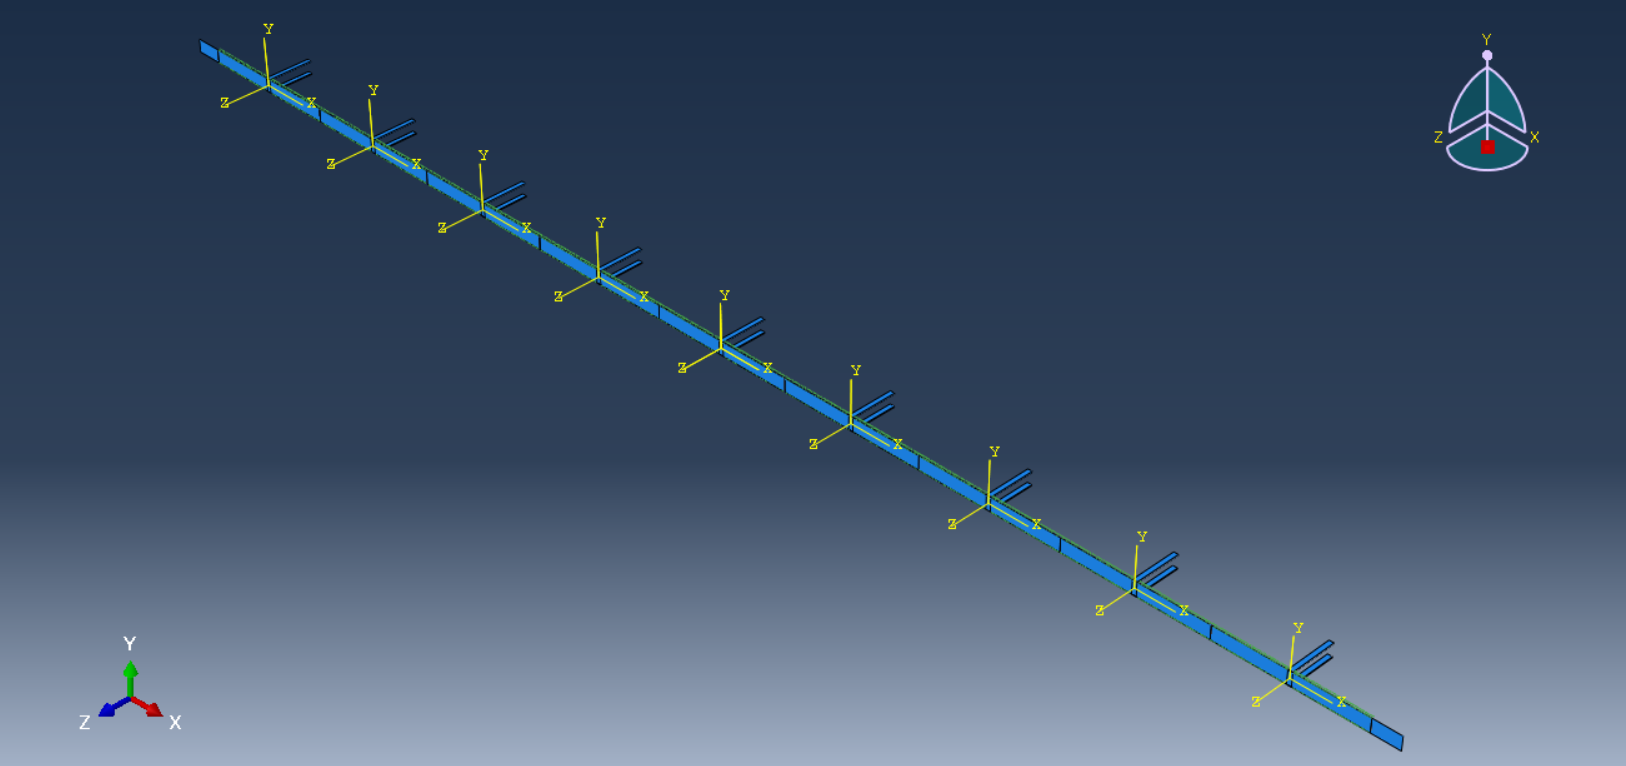
\includegraphics[scale=0.3]{3_1_1.png}

图3.1.1 梁桥整体形态

\subsection{零件设计}

本梁桥采用多跨结构,具有多个全同结构。在abaqus中建模时首先对一个部分进行建模,之后在新的模型中导入多个单体模型再加上边界的桥墩形成整桥。单体结构如图3.1.1.1。

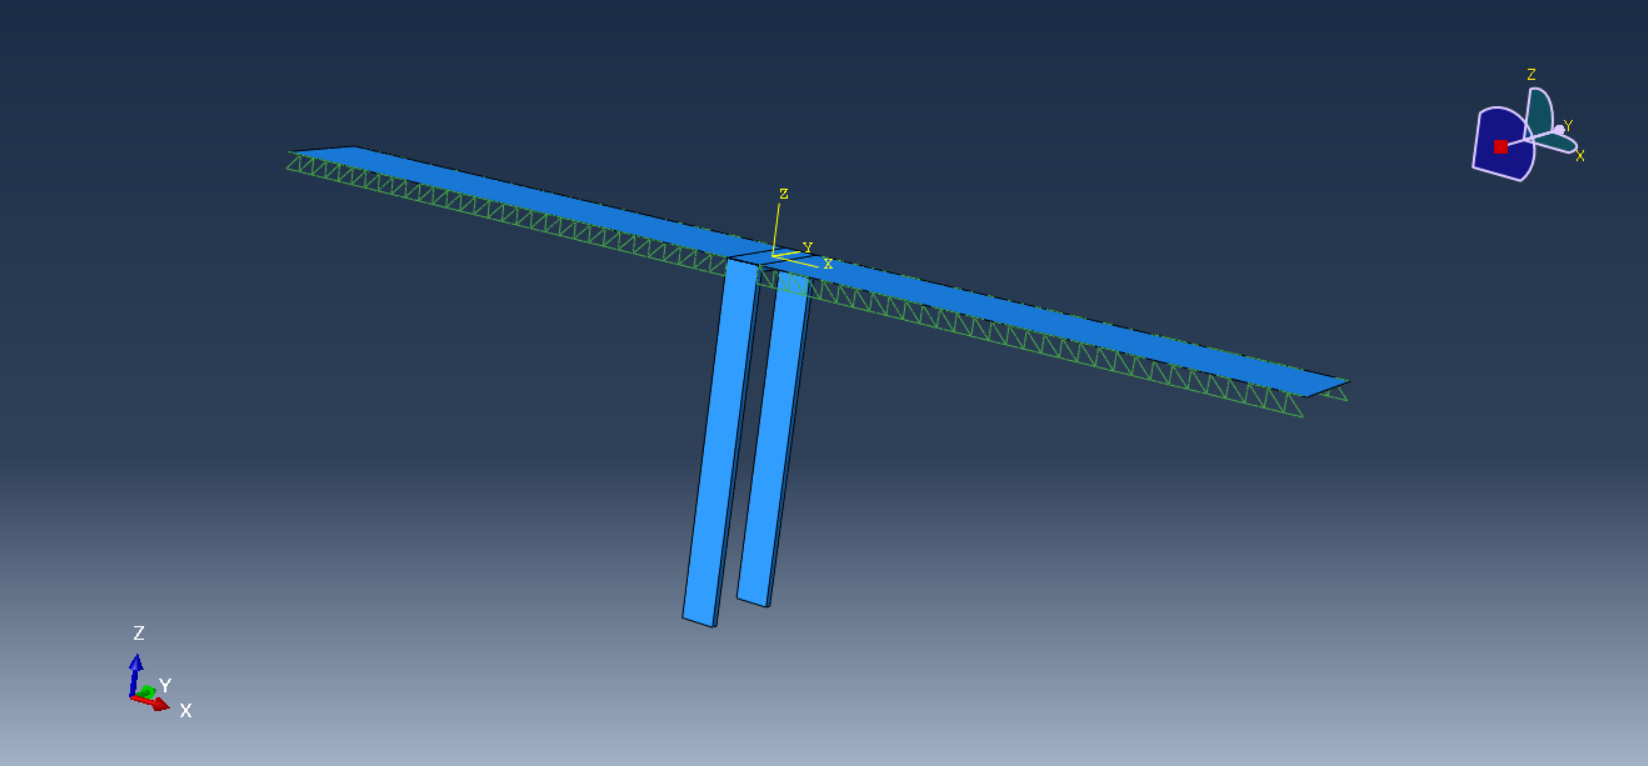
\includegraphics[scale=0.3]{3_1_1_1.png}

图3.1.1.1 单元体模型

每个单体由一个160m长的桥板、一根桥墩和4根半上承梁组成。半上承梁的整体结构如图3.1.1.2。

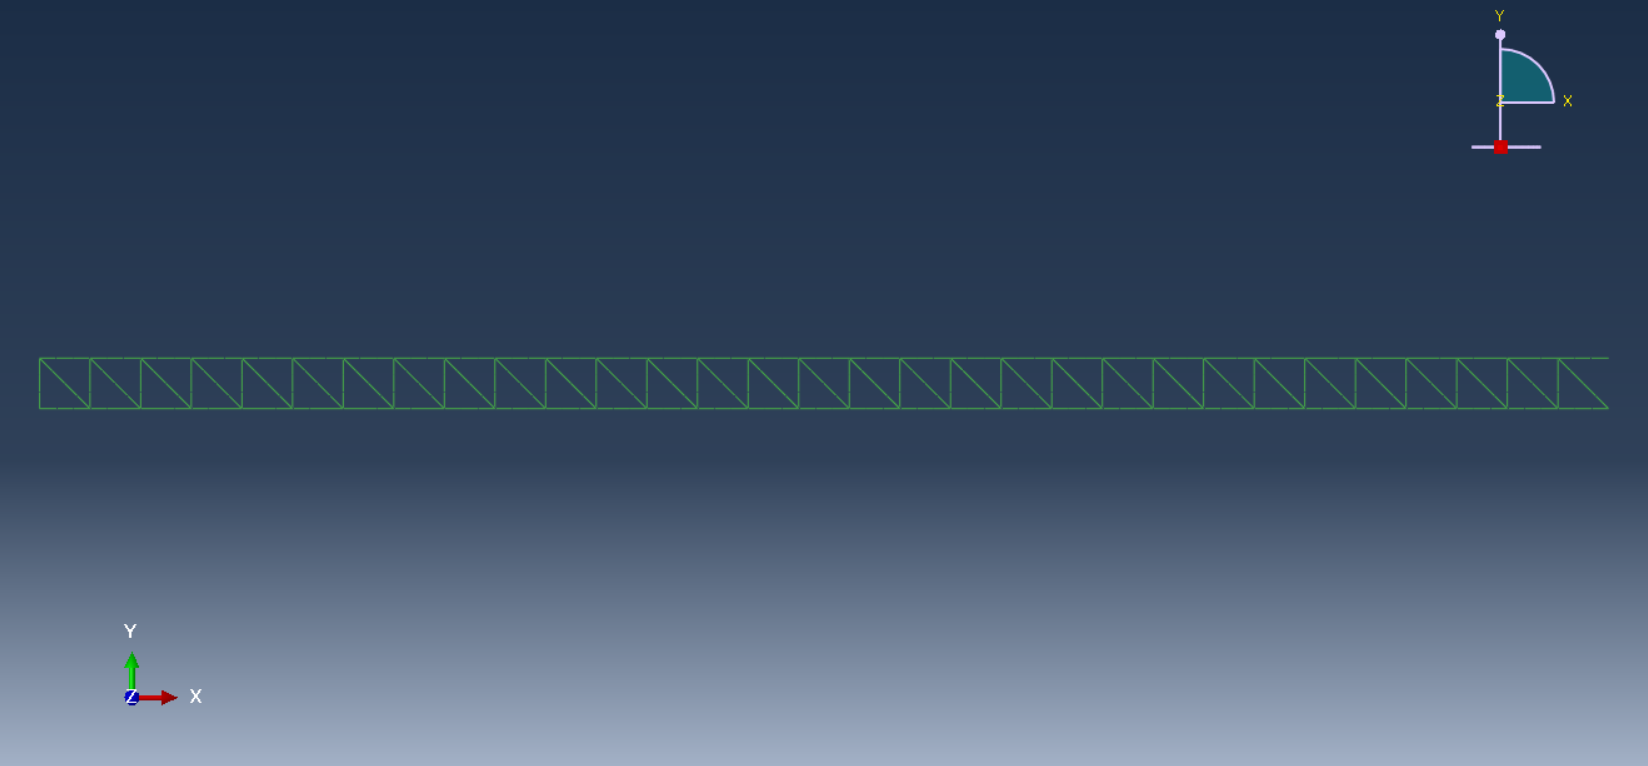
\includegraphics[scale=0.3]{3_1_1_2.png}

图3.1.1.2 半上承梁结构图

每个半上承梁由31个单元体组成,两根半上承梁相对安装形成整根上承梁。上承梁截面采用箱形结构,尺寸如图3.1.1.3。

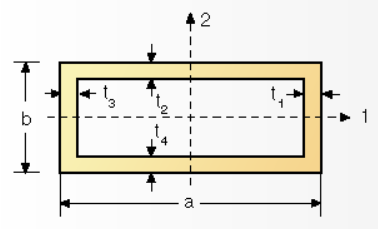
\includegraphics{3_1_1_3.png}

图3.1.1.3 上承梁截面

箱形结构的比刚度较大,相比于工字梁抵抗剪切的能力更强。材料方面,桥面和桥墩选择钢筋混凝土材料,实际施工时需要先编织钢筋再浇筑混凝土。由于stap++不支持复合材料,故这里采用混凝土材料代替(混凝土的抗拉能力要远远低于复合材料钢筋混凝土)。箱形梁使用钢材料(给定的钢材料强度比一般的结构钢大很多)。由于给定材料与实际工程差异比较大,零件的设计也与实际工况有很大的差别。

\subsection{单元类型选择}

梁结构采用三维梁单元B31,对应stap++中的beam单元;桥面采用完全积分的壳单元S4,对应stap++的shell单元;桥墩采用完全积分的实体单元C3D8,对应stap++的8H单元。

\subsection{单元尺寸选择}

单元尺寸按照在应力不超过许用应力的前提下将尺寸尽可能做小的原则选取。由于桥的整体尺寸不便于优化,选择箱形梁的截面参数厚度$b$、宽度$a$、壁厚$t$以及板的厚度$h$进行优化。人工优化结果为:$b=1.5$,
$a=1.5$, $t=0.2$, $h=2$(单位:m)。

\subsection{连接及约束添加}

该桥梁结构复杂,连接关系可以大体分为三类,包括九个全同单元体内部的连接,单元体之间的连接以及主体与边界的连接。单元体内部的连接包括梁与桥板的连接、桥板与桥墩的连接以及梁与桥墩的连接;单元体之间的连接包括相邻桥板、相邻梁、相邻梁与桥板之间的连接。abaqus实现时首先在对单元体建模时将需要连接的部分存入set中,组装整体是调用model可以继承原有model的set,然后直接对set施加连接即可。连接时需要注意一个点集不可以两次作为从面,否则会报错。因此在添加连接时要按照一定规律完成。连接关系全部选择为tie。考虑到stap++没有铰接功能,在选项中勾选锁定转角以保证和stap++一致(实际工程肯定不是这样,单纯是为了对照方便)。约束条件定义为所有桥墩的地面三个方向位移为0,;加载为桥面均匀加载10000Pa。考虑到stap++只能处理点集的连接关系和约束,这里的所有set均选择点集,这也导致几何关系和网格必须协调,降低了优化性能。

\subsection{结果}

结果见图3.1.5.1及图3.1.5.2,最大位移为1.78m,桥墩的应力超过了许用应力,下一步需要更粗的桥墩来适应应力。这也符合梁桥承载能力有限的特点。

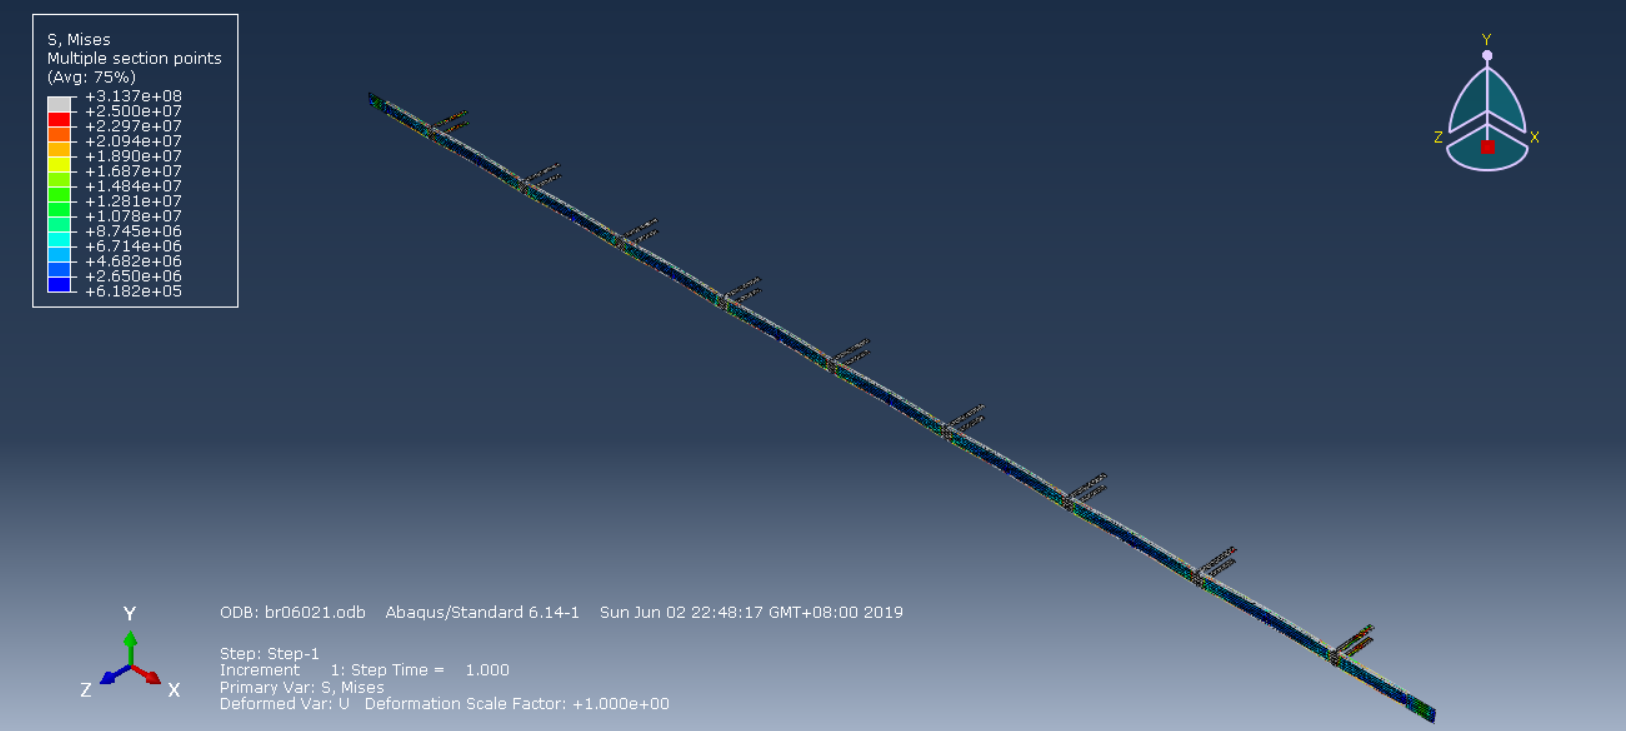
\includegraphics[scale=0.3]{3_1_5_1.png}

图3.1.5.1 梁桥Mises应力云图

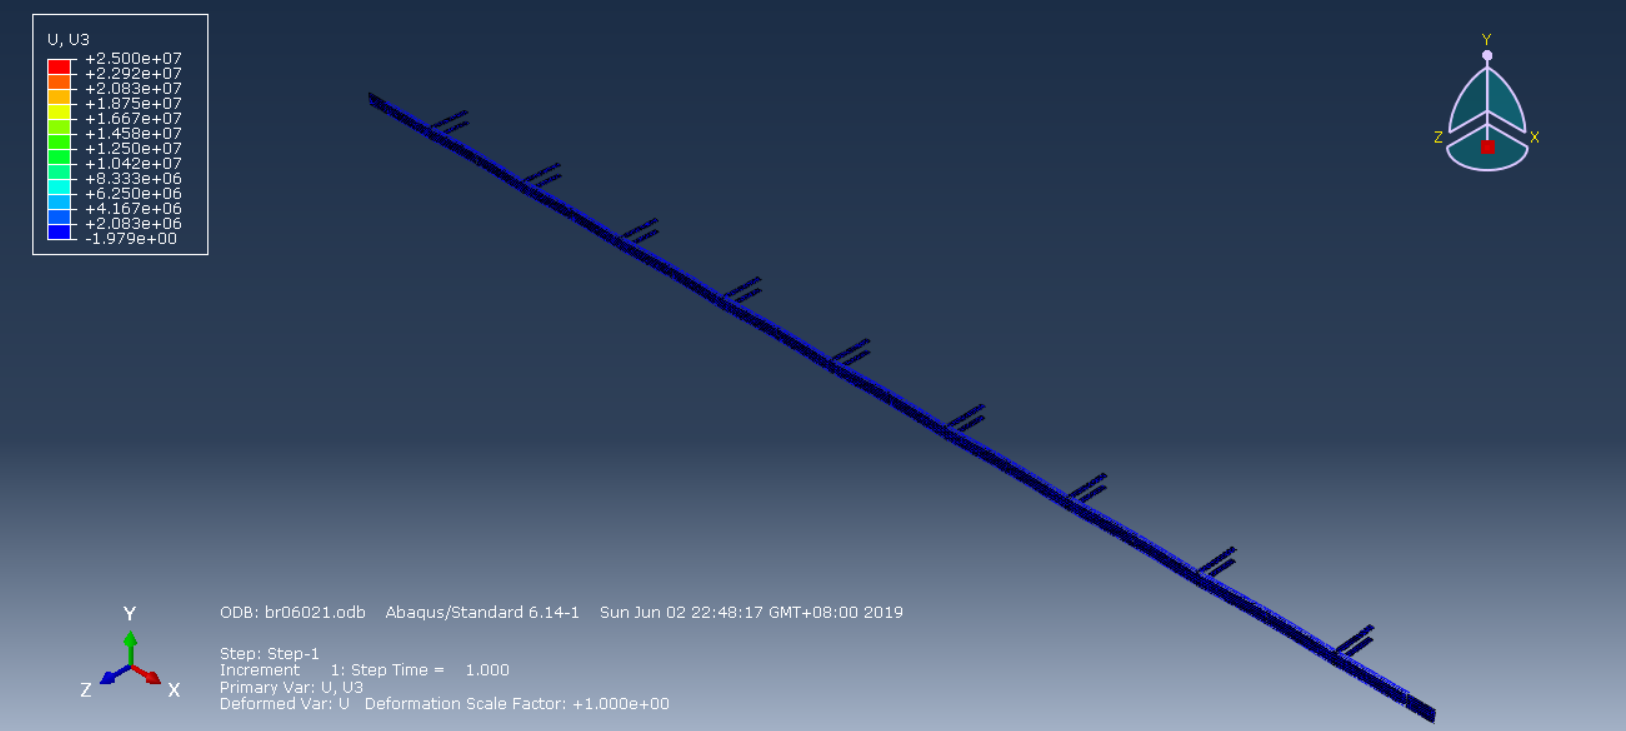
\includegraphics[scale=0.3]{3_1_5_2.png}

图3.1.5.2 梁桥z方向位移云图

\chapter{桥梁的cost计算}

\section{Abaqus-Python脚本读取过程}
在桥梁的大体结构设计确定之后,在进行几何参数改良时,如果在CAE界面改参数将变得非常繁琐,而将模型进行python录制后直接读入相关参数进行计算将非常方便;与此同时,由于我们最终需要集中优化的参数为桥梁的最大位移,桥梁的总造价和承载应力情况,而CAE界面只能查看应力的大体分布情况,无法对所有单元的应力分布情况做一个具体的分析,因此我们还需要利用python脚本对整个Abaqus数据结构进行有选择性的数据读取,其中主要包括节点位移,单元应力,以及单元对应的高斯点坐标,单元几何属性等;与此同时我们可以利用matlab等软件作为python的外部接口,即为python脚本提供输入数据(inp文件),并对输出数据进行相应的分析。整个脚本的程序逻辑结构如图\ref{4-1}所示:

\begin{figure}[H]
\centering  
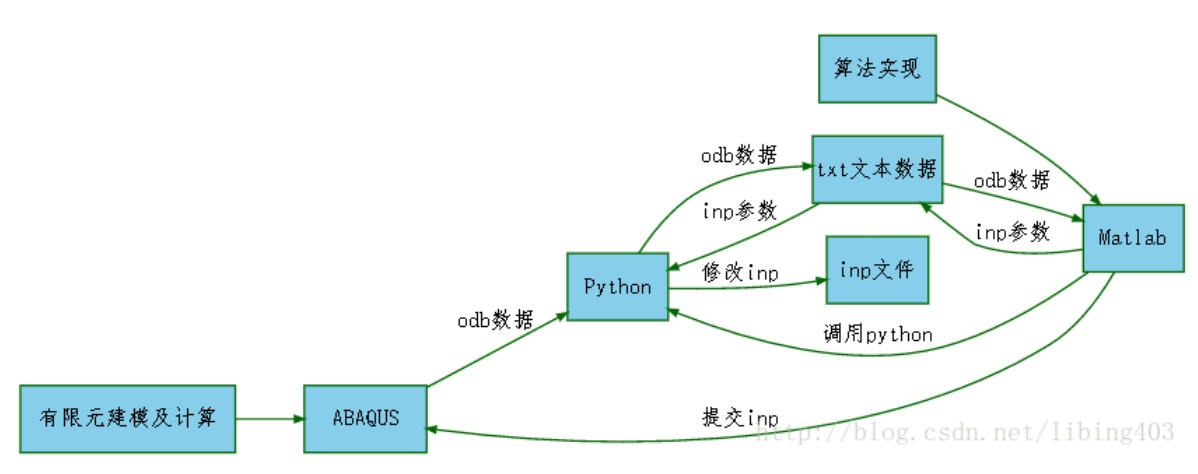
\includegraphics[width = .8\textwidth]{1.png} 
\caption{python后处理设计逻辑} 
\label{4-1} 
\end{figure}

\subsection{ODB对象数据结构:}

如图\ref{4-2}所示:ODB对象主要对包含计算模型对象数据(Model Data)和计算结果数据(Result Data),计算模型对象数据包含装配体(rootAssenbly)
、零件(parts) 、界面分类(sectionCategories)、材料(materials) 等子对象,计算结果数据steps包含分析步(step)
、帧(frame) 、历史变量输出(historyoutputs) 和场变量输出(field outputs) 等。场变量的读取路径:odb.Setps{[}{]}.frames{[}{]}.fieldOutputs{[}{]};

场变量包括:应力分量-'S';应-'E'; 位移-'U';

历史变量的读取路径:odb.Setps{[}{]}.historyRegions{[}{]}.historyOutputs{[}{]};

\begin{figure}[H]
\centering  
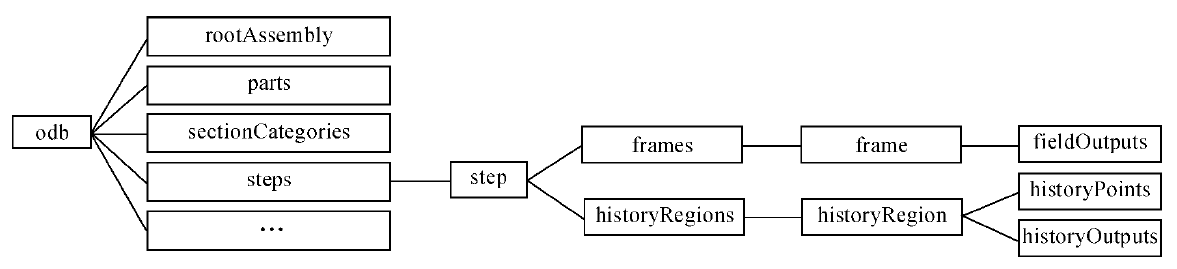
\includegraphics[width = .8\textwidth]{2.png} 
\caption{Abaque odb数据结构示意图} 
\label{4-2} 
\end{figure}

\subsection{MDB对象数据结构}

如图\ref{4-3}所示:MDB对象主要对包含计算模型对象数据(Model Data) 和工作对象数据(Job Data) ,其中model对象,包含零件(parts)
、材料(materials) 等子对象。零件(parts) 子对象包含单元(elements) 、集合(sets) 和节点(nodes)
子对象,其下又包含编号(label) 、坐标(coordinate) 、单元所属节点组(connectivity)等属性。

几何集的读取路径:mdb.models{[}{]}.parts{[}{]}.sets{[}{]}.odb.rootAssembly.instance{[}{]}.elementSets{[}{]};

几何集所属单元,节点信息读取路径:

单元编号:mdb.models{[}{]}.parts{[}{]}.sets{[}{]}.elements{[}{]}.elementLabel.odb.rootAssembly.Instances{[}{]}.elementSets{[}{]}.elements{[}{]}.
elementLabel;

单元所属节点组:mdb.models{[}{]}.parts{[}{]}.sets{[}{]}.elements{[}{]}.Connectivity.odb.
rootAssembly.instances{[}{]}.elementSets{[}{]}. elements{[}{]}. connectivity;

节点坐标:mdb.models{[}{]}.parts{[}{]}.sets{[}{]}.nodes{[}{]}.coordinates;

\begin{figure}[H]
\centering  
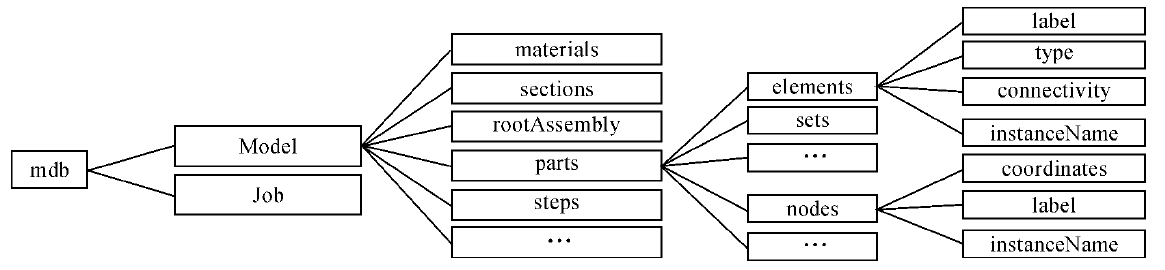
\includegraphics[width = .8\textwidth]{3.png} 
\caption{Abaque mdb数据结构示意图} 
\label{4-3} 
\end{figure}

\subsection{最大位移读取}

我们在odb对象中把位移场’U’的数据读取出来,然后对节点进行循环得到最大的位移数值,如图\ref{4-4}所示:

\begin{figure}[H]
\centering  
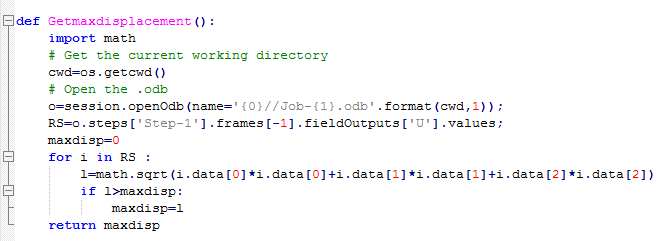
\includegraphics[width = .8\textwidth]{4.png} 
\caption{最大位移读取程序示意图} 
\label{4-4} 
\end{figure}

\subsection{单元应力和最大许用应力}

首先先在odb对象中把应力场’S’中的数据读取出来,然后再将其写入txt文件中,同时输入相应的单元类型和单元号,以便之后对应相应的单元属性,如图\ref{4-5}所示:

\begin{figure}[H]
\centering  
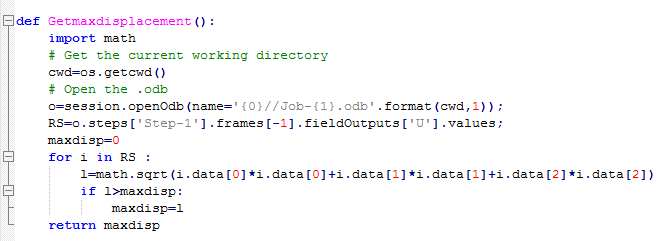
\includegraphics[width = .8\textwidth]{4.png} 
\caption{应力读取程序示意图} 
\label{4-5} 
\end{figure}

\subsection{单元属性读取}

最后我们在mdb对象中得到所有单元的材料属性和坐标等参数,写入到另一个txt文件中,如图\ref{4-6}所示:

\begin{figure}[H]
\centering  
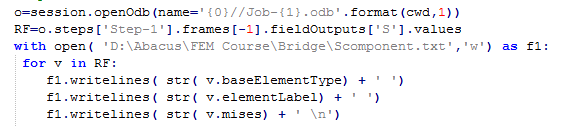
\includegraphics[width = .8\textwidth]{5.png} 
\caption{单元属性读取程序示意图} 
\label{4-6} 
\end{figure}

之后再将相关的单元应力和单元信息参数一同导入到matlab中进行相关的循环检索,利用超过许用应力的单元对应到其单元类型,利用其单元数据计算出其体积;最后检索所有的单元信息得到所有单元的体积总和,一方面计算相应的参数

\chapter{桥梁的优化过程}
对于桥梁优化的整体指标为竞赛说明文件中所述的cost function为
\begin {equation} 
\Pi_{i}=\sqrt{0.4\left(\frac{d_{i}}{a_{1, i}}\right)^{2}+0.4\left(\frac{p_{i}}{a_{2, i}}\right)^{2}+0.2\left(\frac{v}{a_{3, i}}\right)^{2}}
 \end {equation}
其中$d_i$为桥梁平面的最大位移。同时记单元中有$\frac{3}{4}$高斯点在测试工况下达到许用应力的0.8倍的单元为危险单元。$p_i$反应了危险单元体积占整体单元体积的比例。\par
由于无从知晓其他组的各个指标,我们假设各组的指标间的比例关系与我们类似,所以我们的优化过程中简单的将代价函数替换为
\begin {equation} 
\Pi_{i}=\sqrt{0.4\left(\frac{d_{i}}{b_{1, i}}\right)^{2}+0.4\left(\frac{p_{i}}{b_{2, i}}\right)^{2}+0.2\left(\frac{v}{b_{3, i}}\right)^{2}}
 \end {equation}
将原有的分母部分改成遗传算法中出现的分项指标的最大值。将此作为我们的优化目标。\par
整体的优化思路为,首先选取不同样式的桥,分析桥的构型,确定基本设计方案,以及设计方案中的可变参数,其次通过Abaqus的Python脚本接口,参数化的生成桥,之后同样通过Python脚本导出相关的各项指标,如桥面最大位移,以及危险单元占比,之后将桥的相关参数及各项指标导入优化算法,计算出最终的cost,同时分析计算出下一步的各项参数,在Abaqus中画出桥,并计算cost,之后不断迭代,达到指定步长后提取出全局最优解及相关参数。
\section{算法的选择}
\subsection{离散与连续}
算法的选择上有两个层面的选择问题,一是离散和连续算法的选择,二是确定不同种类的离散或连续算法。首先对各项指标分析,工程造价这一项指标可以比较显示的表达成不同单元体积与材料成本的乘积,但桥面最大位移,以及危险单元占比可能很难显示的表达,因此整体的代价函数中有一部分为有解析描述另一部分无解析描述。单纯采用连续的算法并不可行,此时可以采取的思路包括,采取分裂算子的思路,将连续指标与离散指标分裂开来,分部的优化迭代,但分裂算子方法较为复杂,同时对于纯离散问题,算子分裂也并没有成熟稳定的解决方案,因此我们选择了最后一种方案,即将整题的问题考虑为一个离散问题,直接用离散方法对其求解。\par
\subsection{离散算法的选择}
模拟退火算法具有摆脱局部最优解的能力,能够以随机搜索技术从概率的意义上找出目标函数的全局最小点。但是,由于模拟退火算法对整个搜索空间的状况了解不多,不便于使搜索过程进入最有希望的搜索区域,使得模拟退火算法的运算效率不高。模拟退火算法对参数(如初始温度)的依赖性较强,且进化速度慢。\par
遗传算法具有良好的全局搜索能力,可以快速地将解空间中的全体解搜索出,而不会陷入局部最优解的快速下降陷阱;并且利用它的内在并行性,可以方便地进行分布式计算,加快求解速度。但是遗传算法的局部搜索能力较差,导致单纯的遗传算法比较费时,在进化后期搜索效率较低。\par
综上所述,结合了此处桥梁设计问题的特点,以及算法的效率和可行性分析,因为结果随参数的波动可能较为剧烈,为较快的搜索到全局最优解的邻域,我们选取了遗传算法。
\section{遗传算法的简介}
生物在漫长的进化过程中,从低等生物一直发展到高等生物。这是自然环境选择的结果。人们研究生物进化现象,总结出进化过程包括复制、杂交、变异、竞争和选择。一些学者从生物遗传、进化的过程得到启发,提出了遗传算法(GA)。算法中称遗传的生物体为个体,个体对环境的适应程度用适应值表示。适应值取决于个体的染色体,在算法中染色体常用一串数字表示,数字串中的一位对应一个基因。一定数量的个体组成一个群体。对所有个体进行选择、交叉和变异等操作,生成新的群体,称为新一代。\par
遗传算法属于进化算法Evolutionary Algorithms的一种,它通过模仿自然界的选择与遗传的机理来寻找最优解。遗传算法有三个基本算子:选择、交叉和变异。数值方法求解这一问题的主要手段是迭代运算。一般的迭代方法容易陷入局部极小的陷阱而出现"死循环"现象,使迭代无法进行。遗传算法很好地克服了这个缺点,是一种全局优化算法。\par
\section{程序设计思路}
\subsection{编码}
(1)选择合适的编码方案,将各参量拼接转换为染色体。联系实际问题,为每个待优化的变量规定上界与下界,如桥墩的间隔这一参数就小于河床的宽度,大于要求的至少150m。之后确定每个参量的基因组长度,即其离散的密度和优化的精度,对于二进制编码,优化的精度为$\frac{t_{upper-limit}-t_{lower-limit}}{2^n}$。将上下限中的点等分,对应到二进制编码中。\par
(2)选择合适的参数,包括每一步迭代中的群体大小、交叉概率$P_{crossover}$和变异概率$P_{mutation}$\par
(3)确定适应值函数$f(x)$,考虑到这里的适应值为正值,所以对cost函数取相反数之后加上一个常数即可。
\subsection{初始化} 
在最开始的桥的基础上,提取出参数,同时施加一些扰动。将这些作为第一代群体的一部分,另一部分由简单的随机染色体组成,这样既保证了合理解的邻域附近比较全面的搜索,同时完全随机的染色体也保证了群体的基因多样性。初始解的存在保证了优化算法的结果一定是优于最开始的计算结果。
\subsection{繁衍}
\subsection{交叉}
(1)对每串产生[0,1]间随机数,若r>pc,则该串参加交叉操作,如此选出参加交叉的一组后,随机配对。\par
(2)对每一对,产生[1,m]间的随机数以确定交叉的位置。\par
 (3) 将一对染色体m点后的位置互换
\subsection{变异}
如变异概率为Pm,则可能变异的位数的期望值为Pm ×m×M,每一位以等概率变异。具体为对每一串中的每一位产生[0,1]间的随机数r,若r<Pm,则该位发生反转,如对染色体二进制编码为数字0变为1,1变为0。对群组不断进行变异和交叉互换操作,直到下一群体中个体数目达到所要求的M。
\subsection{选择}
对群体中每一染色体(串)计算其适应值,同时计算群体的总适应值。计算每一串的选择概率$Pi=\frac{fi}{F}$及累计概率。选择一般通过简单的古典概型描述,产生[0,1]间随机数r,根据r所在区间选取对应的染色体个体。
\subsection{算法总结}
由于选择概率是由适应值决定的,即适应值大的染色体入选概率也较大,使选择起到"择优汰劣"的作用。交叉使染色体交换信息,结合选择规则,使优秀信息得以保存,不良信息被遗弃。变异是基因中得某一位发生突变,以达到产生确实有实质性差异的新品种。遗传算法虽是一种随机算法,但它是有导向的,它所使用的"按概率随机选择"方法是在有方向的搜索方法中的一种工具。正是这种独特的搜索方法,使遗传算法自然地避开了其它最优化算法常遇到的局部最小陷阱。\par
遗传算法与传统的优化方法(枚举,启发式等)相比较,以生物进化为原型,具有很好的收敛性,在计算精度要求时,计算时间少,鲁棒性高等都是它的优点。
\section{优化实例}
对于这一优化算法我们选取了简单的示例进行验证,简单考虑一个悬索斜拉桥,具体的参数包括桥墩的跨度,每个支架所对应的悬索根数,桥墩的尺寸,悬索的面积。简单基于悬臂梁的推导,$d\propto x^4,M\propto x^2,M\propto \sigma_{max}^2,n \propto L^{-1}$。我们可以发现桥墩的跨度与桥面最大位移成四次方关系,假设单元的最大应力值呈线性分布,因此与危险单元占比个数呈二次方关系,与造价成反比关系。对于悬索根数,$d \propto L^4,L \propto n^{-1}$,可以推出$d \propto n^{-4}$,与桥墩跨度类似,与危险单元个数呈负二次方关系,与造价成正比。桥墩的尺寸与悬索的截面积均与造价成正比,考虑其对危险单元个数与桥面最大位移影响不大。
\begin{figure}[H]
\centering
    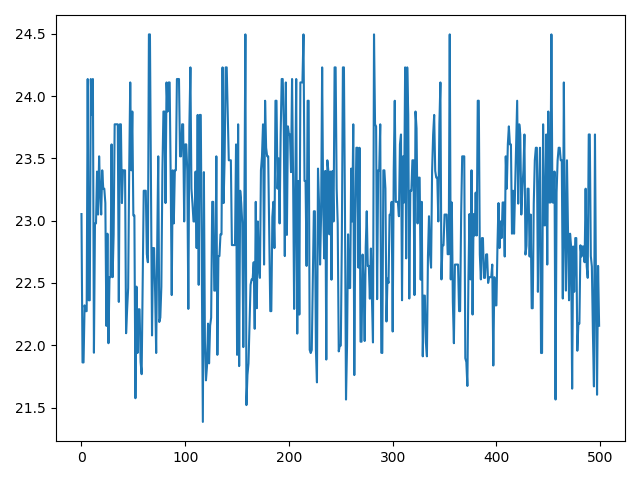
\includegraphics[width=.9\textwidth]{GA.png}\hfill
  \caption{Symmetry and asymmetry lines and Boudary condition}
\label{fig:1}
\end{figure}
优化结果如图所示,选取的桥梁跨度为160m,选取的悬索根数(每段)52。

%\bibliographystyle{plain}
%\bibliography{bridge_report}
\cleardoublepage
\end{document}

%%%============================================================================================================%%%

%%%=== 参考文献 ========%%%




